\section{模块 4 · 步骤 2 下篇：把粘连的楼拆开——marker 分水岭与碎片吸收}

模块 3 结束时，我们有了一批初步楼块，其中一部分仍然``一块粘着好几栋楼''：
有的楼确实靠得太近，0.5 米格子上只隔一两格；有的被零星错点或伸过来的树枝搭了桥。
闭运算已经被我们废掉了，这些粘连不是闭运算造成的，
而是\textbf{真实数据里就存在的接触}。本模块解决两个问题：
\textbf{怎么发现}哪些块粘着多栋楼？\textbf{在哪里下刀}把它们分开？

\subsection{发现粘连：腐蚀取``核''}

工具还是模块 3 介绍过的\textbf{腐蚀}（黑色区域向内削一圈），但这次拿它当探测器用。
对每个楼块，用半径 1.5 米的圆盘做腐蚀——把块的边界向内削掉 1.5 米。直觉是：

\begin{itemize}
\item 一栋正常的楼（宽 8--15 米）削掉一圈后，中间还剩一大块——剩下的部分叫\textbf{核（core）}；
\item 两栋楼若只靠一条\textbf{窄于约 3 米}的``细脖子''相连（两侧各削 1.5 米），
      削完后脖子断开，剩下\textbf{两个分离的核}；
\item 削剩的零星小渣不算核——核的面积必须 $\geq 6$ 平方米才算数
      （否则屋顶边缘的毛刺也会被当成``第二栋楼''）。
\end{itemize}

于是判据非常干净：\textbf{一个块腐蚀后剩几个合格的核，就估计它里面有几栋楼}。
合格核不足 2 个的块（剩 1 个核，或窄楼被整个削没、0 个核）一律不拆、原样保留；
出现 $\geq 2$ 个核的块被送进下一小节拆分。顺带把单位换算清楚：
$6$ 平方米 $= 24$ 个 $0.5$ 米格子，门槛取在``明显小于最小目标建筑
（20 m\textsuperscript{2}）、又远大于边缘毛刺''的位置。

\begin{figure}[H]
\centering
\begin{tikzpicture}[scale=0.55]
% 原块：两矩形+细脖子
\begin{scope}
\fill[blue!40] (0,0) rectangle (4,3);
\fill[blue!40] (6,0.2) rectangle (10,3.2);
\fill[blue!40] (4,1.2) rectangle (6,2.0);
\node[font=\small] at (5,-0.9) {一个连通域：两栋楼被``细脖子''连着};
\end{scope}
% 腐蚀后
\begin{scope}[xshift=12.5cm]
\fill[blue!40, opacity=0.25] (0,0) rectangle (4,3);
\fill[blue!40, opacity=0.25] (6,0.2) rectangle (10,3.2);
\fill[blue!40, opacity=0.25] (4,1.2) rectangle (6,2.0);
\fill[blue!80] (0.75,0.75) rectangle (3.25,2.25);
\fill[blue!80] (6.75,0.95) rectangle (9.25,2.45);
\node[font=\small, blue!60!black] at (2,2.7) {核 1};
\node[font=\small, blue!60!black] at (8,2.9) {核 2};
\node[font=\small] at (5,-0.9) {腐蚀 1.5 m 后：脖子断了，剩两个核};
\node[font=\small] at (5,-1.7) {$\Rightarrow$ 判定``这块里有两栋楼''};
\end{scope}
\end{tikzpicture}
\caption{腐蚀取核：窄于约 3 米的连接经不起两侧各削 1.5 米；核的个数用于估计楼的栋数。}
\label{fig:erosion-core}
\end{figure}

\subsection{在哪里下刀：marker 分水岭}

知道了``这块里有两栋楼''，还得决定\textbf{分界线画在哪}。这时高度信息登场了
——模块 3 栅格化时，我们给每个格子存了``格内最高点高程 $z_{\max}$''，
现在它拼成一张\textbf{高度图}。关键观察：

\begin{center}
\fbox{\parbox{0.92\textwidth}{\centering
两栋楼即使在平面上粘着，\textbf{接缝处的高度通常塌下去}：
屋顶是块内最高的地方，而楼间的间隙里多半只有矮灌木、栅栏、地面或搭桥的零星点
——沿着``从一栋楼走到另一栋楼''的路径看高度，中间通常有一段\textbf{低谷}。
理想的分界线，就应该沿着这条高度低谷走。说``通常''而不说``必然''是有分寸的：
若伸进缝里的树枝比屋檐还高、或零星高错点把低谷抬了起来，低谷会变浅甚至消失，
边界就可能切偏——这类残余错误由人工抽查和模块 6 的``缝内地面命中''仲裁兜底。
}}
\end{center}

\textbf{分水岭算法（watershed）}正是把这个直觉自动化的经典工具（模块 2 提到的
Beucher \& Meyer 1993）。它把一张图当作\textbf{地形}来看，往里灌水：
水从各个盆地底部涨起，水位同步上升，\textbf{两片来自不同盆地的水相遇时，
在相遇处筑一道坝}——所有的坝连起来就是分割边界。

两个实现细节（也是导师可能追问的点）：

\textbf{（a）为什么用 $-z_{\max}$（高度取负）当地形？}
分水岭在``盆地''里灌水、在``山脊''上筑坝。我们想要的边界在\textbf{高度低谷}，
所以把高度整体取负、上下翻转：翻转后，高高的屋顶变成了深盆地（水源所在），
楼间低谷翻成了山脊——坝沿着山脊筑，即\textbf{边界倾向沿两楼之间高度较低的分隔带走}
（在平坦或有噪声的地方，坝的位置会有几个格子的摆动，不保证严格踩在绝对最低点的连线上）。

\textbf{（b）为什么要 marker（指定水源）？}
经典分水岭让\textbf{每一个}局部洼地都自己冒水，屋顶上随便一个烟囱、一段屋脊造成的
小起伏都会多出一片水——结果是块被切得粉碎（过分割）。
\textbf{marker 控制版}只允许指定的位置冒水：我们把上一小节的\textbf{核}当水源，
几个核就几片水，块的\textbf{主体}恰好按核数分开。两个补充细节：
其一，灌水范围被限制在原块内部（外面不归它管）；
其二，补洞补出来的格子没有点、也就没有实测高度，程序把它们赋成``极高的隔墙''参与灌水
——水最后才漫过去，通常顺势并入相邻水域；万一存在完全被隔死、水到不了的死角，
程序不强行分配，给它单独编号（实践中极少发生）。

\begin{figure}[H]
\centering
\begin{tikzpicture}[scale=0.75]
% 高度剖面
\draw[->] (0,0) -- (13.2,0) node[right,font=\small] {沿剖面位置};
\draw[->] (0,0) -- (0,3.6) node[above,font=\small] {高度 $z_{\max}$};
\draw[thick, blue!70!black]
  (0.3,0.4) -- (1.0,2.6) -- (2.6,3.0) -- (4.4,2.5) -- (5.4,0.9)
  -- (6.6,0.7) -- (7.6,1.0) -- (8.4,2.8) -- (10.4,3.1) -- (11.8,2.4) -- (12.6,0.5);
\node[font=\small, blue!70!black] at (1.2,3.35) {楼 A 屋顶};
\node[font=\small, blue!70!black] at (11.9,3.45) {楼 B 屋顶};
\node[font=\small] at (6.6,0.28) {楼间低谷（灌木/地面/桥接点）};
\draw[red!70!black, very thick, dashed] (6.6,0) -- (6.6,3.5);
\node[font=\small, red!70!black, align=center] at (6.6,3.85) {分水岭筑坝处 = 分界线};
% 水源标记
\fill[green!60!black] (2.6,3.0) circle (3pt);
\node[font=\scriptsize, green!40!black] at (2.9,2.55) {核 1（水源）};
\fill[green!60!black] (10.4,3.1) circle (3pt);
\node[font=\scriptsize, green!40!black] at (10.1,2.65) {核 2（水源）};
\end{tikzpicture}
\caption{沿``楼 A $\to$ 楼 B''的高度剖面（图中画的是\textbf{原始}高度；
算法实际在上下翻转后的地形上运行——屋顶翻成盆地、低谷翻成山脊）。
水从两个核对应的盆地涨起，相遇即筑坝：坝沿翻转后的山脊、
也就是原始高度的低谷带走。}
\label{fig:watershed}
\end{figure}

\begin{numbox}[：拆分战果]
全区共有 \textbf{168 个}连通域被检出多核并由分水岭拆开
（每次拆分的块号、拆成几份、各份面积都写进了 \texttt{splits\_log.csv} 备查）。
注意归因要分清：这 168 个是 v2 \textbf{自己}检出的多核粘连块——真实贴得近、
树枝搭桥、错点搭桥都在其中；v1 那种闭运算造成的\textbf{人为}焊接已在源头消除，
这里拆的是数据里本来就存在的粘连。168 个块共拆出 383 份、净增 215 个实例。
\end{numbox}

\subsection{防过分割的保险丝：非对称碎片吸收}

去掉闭运算、又对粘连块动刀，代价是偶尔\textbf{矫枉过正}：
屋顶被树冠遮出缺口后剩下的小角、贴着主屋的小门廊，可能孤立成小碎块。
如果放着不管，一栋楼就会变成``一大一小两个实例''（过分割）。
兜底规则是\textbf{碎片吸收}：

\begin{center}
\fbox{\parbox{0.92\textwidth}{\centering
面积 $<20$ m\textsuperscript{2} 的碎片，若在 3 米范围内存在一个面积 $\geq 50$
m\textsuperscript{2} 的``锚''实例，且两者的中位高程差 $\leq 3$ 米，则并入该锚。
}}
\end{center}

三个条件各管一件事：\textbf{面积门槛}保证只有``碎片并整楼''会发生
——两栋各 50 m\textsuperscript{2} 的真实小房子谁也吸收不了谁，
这就是``\textbf{非对称：只许小并大}''的含义，它把吸收机制自己制造欠分割的风险压到最低
（说``最低''而非``零''：一间贴着大楼、高度相近、不足 20 m\textsuperscript{2}
的真实小附属确实会被并入——本项目把这类当作主楼的附属结构，属可接受的取舍，
人工抽查也覆盖这类案例）；\textbf{3 米距离}指碎片到锚实例最近格子的平面距离
（实现上含半格容差；若周围有多个合格的锚，取\textbf{最近}的那一个，无并列歧义）；
\textbf{高程相容}比较两者的\textbf{中位高程}（把各自所有点的高程从小到大排队取正中间那个值
——不被烟囱等零星极端点带偏），拦住``隔着高差硬并''的错误，
例如把 10 米高的树冠碎片并进 4 米高的平房。

\subsection{收尾三件事：丢渣、捡孤儿、发号}

\textbf{（1）丢渣}：吸收后仍孤立、面积 $<20$ m\textsuperscript{2} 的小块按噪声丢弃
——这是项目的\textbf{最小制图面积}取舍：比单车库还小的独立结构
（工具棚、狗屋、凉棚）不在本项目的建模目标内，而零星错点凑成的假团块又恰好多在
这个尺寸段，一刀切最干净。
\textbf{（2）捡孤儿}：模块 3 的占据规则（每格 $\geq2$ 点）丢掉了稀疏格子里的点，
其中有些其实是真屋顶的边缘。现在把这些``孤儿点''挂回平面距离 \textbf{1.5 米}（$=3$ 个格子）内\textbf{最近}的实例格
（距离按格网量取，最近者唯一，不存在并列歧义）；1.5 米内没有实例的，
维持无主（instance\_id = 0），不强行认领。窄缝里两楼几乎等距时，
个别边界点可能挂错家门——这是逐点级的小误差，不改变实例结构，由抽查覆盖。
\textbf{（3）发号}：所有实例按面积从大到小重新编号 1, 2, 3, \dots，
每个点的编号作为新增属性 \texttt{instance\_id} 写回点云文件。

\subsection{结果与人工验收}

\begin{numbox}[：步骤 2 最终产出]
\textbf{2{,}296 个建筑实例}（候选），编号 1--2296，逐点写入
\texttt{buildings\_instances.laz}；随机抽查窗口与 v1 出错点的复查图作为质检产物存档。
对账线索：初步连通域数 $+$ 拆分净增 215 $-$ 吸收合并数 $-$ 丢渣数 $= 2{,}296$；
拆分明细逐块存档（\texttt{splits\_log.csv}），吸收与丢渣的逐项计数在运行日志中，重跑可复现。
\end{numbox}

\begin{warnbox}[：显示上的一个小教训——``防撞色'']
最初把实例编号直接用连续色带显示（编号 1 深蓝、2296 深红、中间渐变），
用户检查时发现\textbf{相邻楼的编号往往相近、颜色几乎一样}，看起来就像``同一个实例''
——白白制造了一场虚惊。之后所有实例一律改用\textbf{随机防撞色}
（每个实例随机挑一个颜色、并保证与邻居不同），并把颜色直接写进点云文件的 RGB 属性列（每个点存红、绿、蓝三个颜色数值），
在支持按 RGB 着色的查看软件里打开即见防撞色，不再依赖软件自选的色带。
这个习惯延续到了管线后面所有输出。
\end{warnbox}

\begin{figure}[H]
\centering
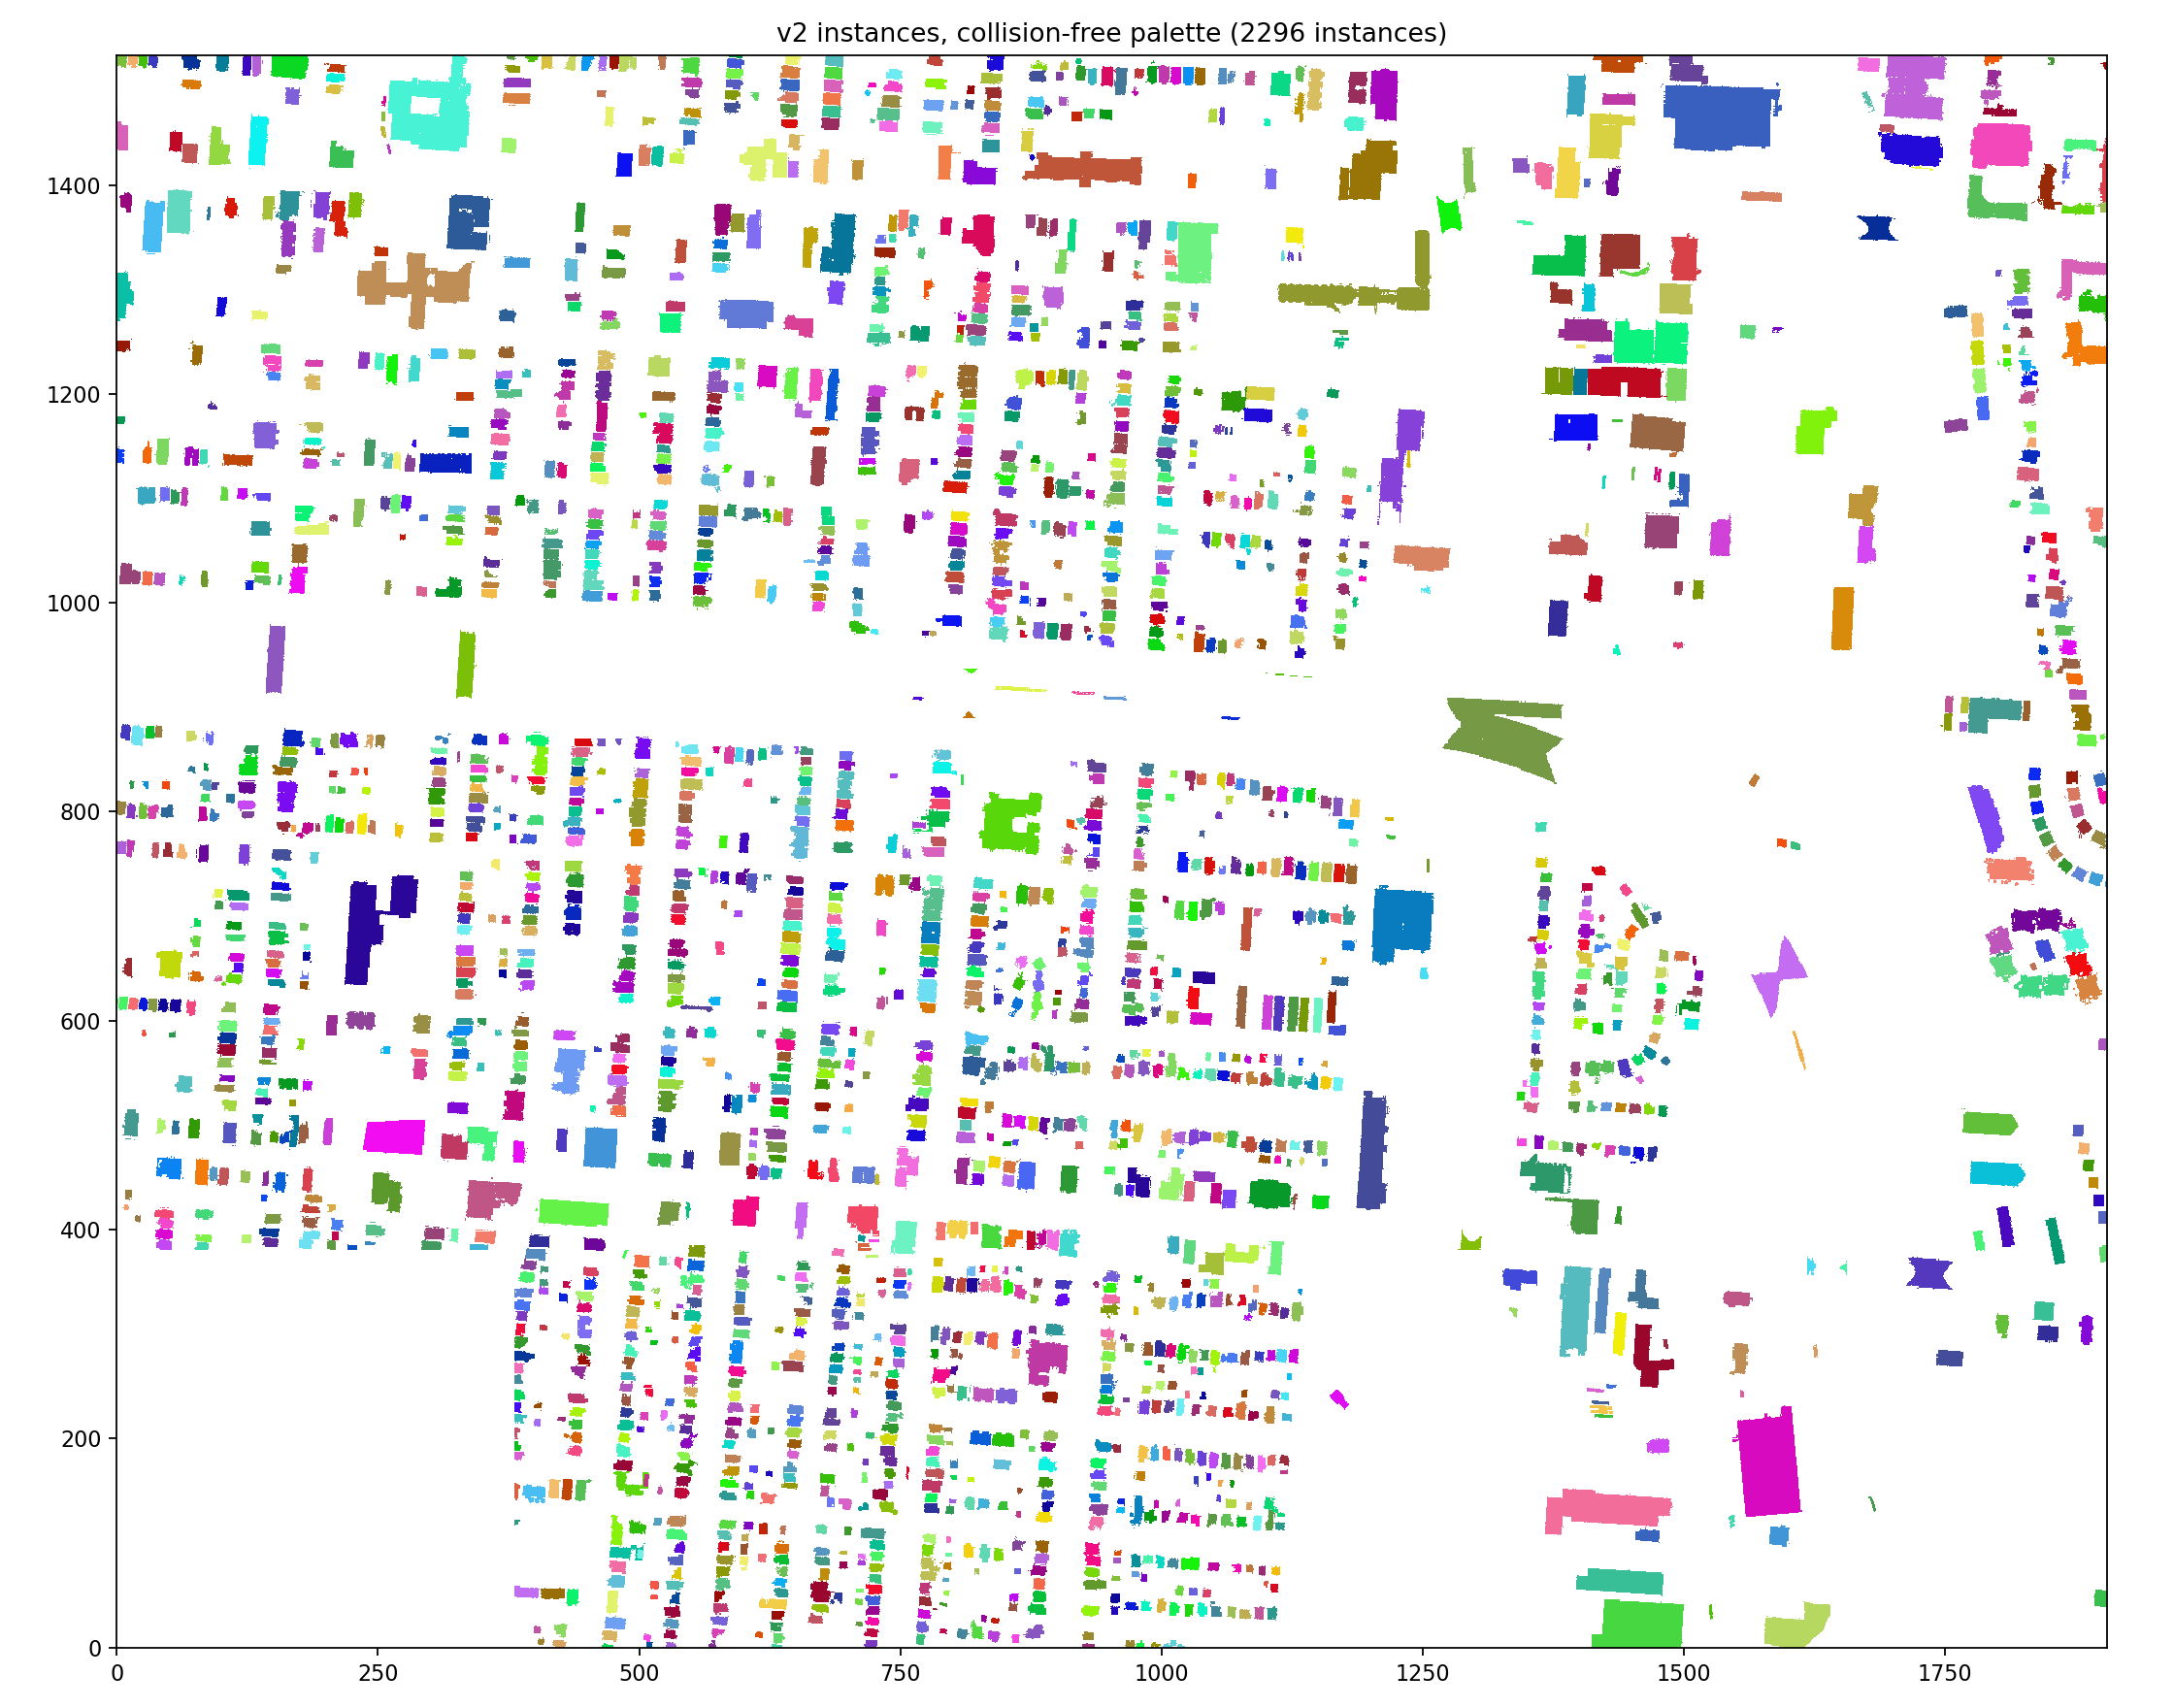
\includegraphics[width=0.9\textwidth]{figs/qa_overview_rgb.png}
\caption{步骤 2 全区总览（每实例一个防撞色）：2{,}296 个候选建筑实例。
可以看到住宅街区被整齐地逐栋分开；图中零星的大块异形目标（桥、匝道等）
正是下一模块 Gate A 要处理的对象。}
\label{fig:overview}
\end{figure}

\begin{plainbox}[：模块 4 小结]
\begin{itemize}
\item 腐蚀取核发现粘连（削 1.5 m、核 $\geq6$ m\textsuperscript{2}），
      168 个多核连通域被 marker 分水岭沿\textbf{高度低谷}拆开（383 份、净增 215）
      ——水源=核，地形=$-z_{\max}$，边界沿两楼之间高度较低的分隔带走。
\item 非对称碎片吸收（$<20$ m\textsuperscript{2} 并入 3 m 内 $\geq50$ m\textsuperscript{2}
      且高程相容的锚）兜住过分割，``只许小并大''保证它不反向制造欠分割。
\item 丢渣、捡孤儿、按面积发号后：\textbf{2{,}296 个候选建筑实例}。
      其中混着的桥、匝道、树冠、电线，交给模块 5 的 Gate A。
\end{itemize}
\end{plainbox}
